\documentclass[12pt]{article}

\usepackage{fullpage}
\usepackage{multicol,multirow}
\usepackage{tabularx}
\usepackage{ulem}
\usepackage{graphicx}%Вставка картинок правильная
\usepackage{float}%"Плавающие" картинки
\usepackage{wrapfig}%Обтекание фигур (таблиц, картинок и прочего)
\usepackage[utf8]{inputenc}
\usepackage[russian]{babel}

% Оригиналный шаблон: http://k806.ru/dalabs/da-report-template-2012.tex

\begin{document}

\section*{Лабораторная работа №\,9 по курсу дискрeтного анализа: графы}

Выполнил студент группы 08-307 МАИ \textit{Дегтярев Денис Андреевич}.

\subsection*{Условие}

Задан взвешенный неориентированный граф, состоящий из n вершин и m ребер. Вершины пронумерованы целыми числами от 1 до n. 
Необходимо найти длину кратчайшего пути из вершины с номером start в вершину с номером finish при помощи алгоритма Дейкстры. 
Длина пути равна сумме весов ребер на этом пути. Граф не содержит петель и кратных ребер.

\subsection*{Метод решения}

Создаем матрицу, которая содержит в себе информацию, посещали ли мы вершину или нет.
Создаем матрицу весов путей, все значения - None.
Стартовую точку заполняем нулем.

Затем для каждой вершины, связанной с начальной ровно $1$ 
ребром проверим, является ли сопоставленное ей в начале число больше, чем 
сумма такого же числа той вершины, из которой мы приши и веса ребра, по 
которому пришли. Если является, заменяем число на эту самую сумму. Как 
только обошли всех соседей вершины, помечаем вершину как пройденную, это 
значит, что минимальное расстояние до этой вершины найдено и изменять его 
больше не надо. То же самое делаем со всеми остальными вершинами, пользуясь 
поиском в глубину.

\subsection*{Описание программы}

Функция dekstra вычисляет стоимость пути к каждой точке и выводит для финиша.

\subsection*{Дневник отладки}  

Тесты пройдены сразу

\subsection*{Тест производительности}

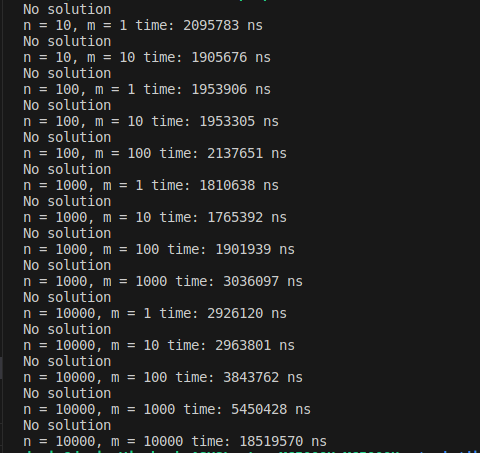
\includegraphics[width=7in]{test.png}

\subsection*{Недочёты}

Недочетов не должно быть... Реализовывал все добросовестно.

\subsection*{Выводы}

Выполнив лабораторную работу №9 по курсу «Дискретный анализ», я изучил
алгоритм Дейкстры и убедился, что он помогает искать все возможные пути
из одной точки графа в другую. Также данный алгоритм позволяет находить кратчайшие пути с определенной точки во все другие точки. 
Это позволяет за вполне разумную временную сложность находить кратчайшие дороги, например, для автобусов. Поэтому алгоритм Дейкстры очень полезен и часто используется до сих пор.

\end{document}
